\documentclass{article}
\usepackage[utf8]{inputenc}
\usepackage{amsmath}
\usepackage{xcolor}
\usepackage{tikz}
\usetikzlibrary{matrix,decorations.pathreplacing, calc, positioning,fit}

\newcommand{\boldU}{\boldsymbol{U}}

\newcommand{\boldSigma}{\boldsymbol{\Sigma}}

\newcommand{\boldV}{\boldsymbol{V}}

\newcommand{\boldJ}{\boldsymbol{J}}

\begin{document}

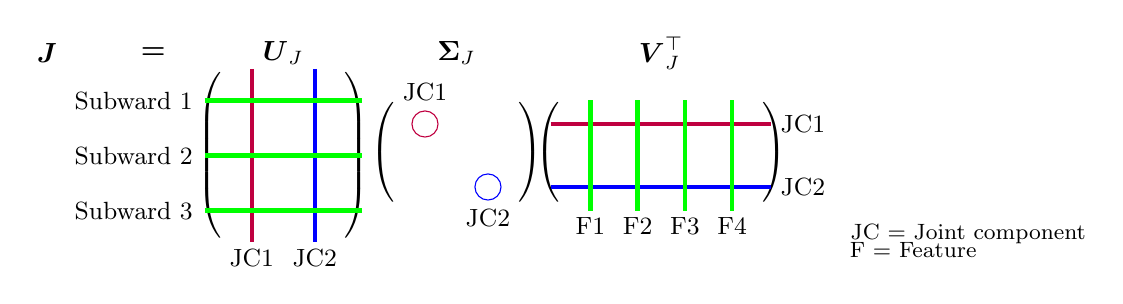
\begin{tikzpicture}%
    \matrix [matrix of math nodes,left delimiter=(,right delimiter=)](U) at (3,0){
        \hspace{1cm} \\
        \hspace{1cm} \\
        \hspace{1cm} \\
        \hspace{1cm} \\
        \hspace{1cm} \\
        \hspace{1cm} \\
        \hspace{1cm} \\
        \hspace{1cm} \\
    };
     \matrix [matrix of math nodes,left delimiter=(,right delimiter=)](Sigma) at (5.2,0){
        \hspace{1cm} \\
        \hspace{1cm} \\
        \hspace{1cm} \\
        \hspace{1cm} \\
    };
     \matrix [matrix of math nodes,left delimiter=(,right delimiter=)](V) at (7.8,0){
        \hspace{2cm} \\
        \hspace{2cm} \\
        \hspace{2cm} \\
        \hspace{2cm} \\
    };
    \draw [ultra thick, purple] (2.6,1.1) to (2.6,-1.1);
    \draw [ultra thick, blue] (3.4,1.1) to (3.4,-1.1);
    \draw [ultra thick, green] (2,0.7) to (4,0.7);
    \node (s1) at (1.1,0.7)
        {\small{Subward 1}};
    \draw [ultra thick, green] (2,0) to (4,0);
    \node (s2) at (1.1,0)
        {\small{Subward 2}};
    \draw [ultra thick, green] (2,-0.7) to (4,-0.7);
    \node (s3) at (1.1,-0.7)
        {\small{Subward 3}};
    \draw [ultra thick, purple] (6.4,0.4) to (9.2,0.4);
    \draw [ultra thick, blue] (6.4,-0.4) to (9.2,-0.4);
    \draw [ultra thick, green] (6.9,0.7) to (6.9,-0.7);
    \node (l1) at (6.9,-0.9)
        {\small{F1}};
    \draw [ultra thick, green] (7.5,0.7) to (7.5,-0.7);
    \node (l2) at (7.5,-0.9)
        {\small{F2}};
    \draw [ultra thick, green] (8.1,0.7) to (8.1,-0.7);
    \node (l3) at (8.1,-0.9)
        {\small{F3}};
    \draw [ultra thick, green] (8.7,0.7) to (8.7,-0.7);
    \node (l4) at (8.7,-0.9)
        {\small{F4}};
    \node[circle, draw=purple] (s1) at (4.8,0.4){};
    \node[circle, draw=blue] (s2) at (5.6,-0.4){};
    \node (uj) at (3,1.3)
        {$\boldU_J$};
    \node (sj) at (5.2,1.3)
        {$\boldSigma_J$};
    \node (vj) at (7.8,1.3)
        {$\boldV_J^\top$};
    \node (j) at (0,1.3)
        {$\boldJ$};
    \node (eq) at (1.35,1.3)
        {$\boldsymbol{=}$};
    \node (j1) at (2.6,-1.3)
        {\small{JC1}};
    \node (j2) at (3.4,-1.3)
        {\small{JC2}};
    \node (j1a) at (9.6,0.4)
        {\small{JC1}};
    \node (j2a) at (9.6,-0.4)
        {\small{JC2}};
    \node (j1b) at (4.8,0.8)
        {\small{JC1}};
    \node (j2b) at (5.6,-0.8)
        {\small{JC2}};
    \node (x1) at (11.7,-1)
        {\footnotesize{JC = Joint component}};
    \node (x1) at (11,-1.2)
        {\footnotesize{F = Feature}};
\end{tikzpicture}

\end{document}